\chapter{NEEM-Hub}
\label{ch:neemhub}
\chapterauthor{S. Koralewski}


With the \neemhub we want to 
neem hub, store data, version control, machine learning access to \openease. 
To implement the version control of large data sets and machine learning models, we are using DVC\footnote{text}\url{https://dvc.org/}. 
We use Hadoop\footnote{\url{https://hadoop.apache.org/}} and its file system HDFS to store the data and models.
Hadoop is a cluster system which creates automatically replicas of the data once it is uploaded and allows parallel processing of data to speed up transforming or querying data.

On a high level perspective we want to realize two pipelines with our \neemhub as depict in Figure \ref{fig:neem-hub}. \todo{Replace with newer and nicer figure}
The first pipeline can be seen as the acquisition and analytic pipeline.
Raw data, such as videos, text and images which 
So called Neemifier should transform this raw data into \neems which are utilizing the semantically representation provided by \soma.
Since we are using Hadoop, multiple instances of the same Neemifier can neemify the raw data in parallel. 
There is also the possibility to upload \neems directly to the \neemhub, so the neemifing step can be skipped.
The stored \neems can be accessed by \openease. \openease allows the inspection and visualization of each individual \neem.
A direct download of the \neems to the local system is also supported.

The second pipeline should be used as a pipeline for learning.
\neems are so rich full on information that one \neem can be used for multiple learning problems.
In addition, \neems allow to learn general models e.g.\ the likely location of perishable items or/and specialized models e.g. how an agent should grasp my favorite mug in my kitchen.
The procedure to generate the models is that Transformers are used to extract the required features from the \neems and store them in a data representation e.g.\ CSV required for the machine learning model.
The Learners, which create the models , store the data in the model library. 
This model library can be used afterwards by an agent to perform reasoning.

In some scenarios those two pipelines can be combined to create a closed-loop. A possible scenario can be a robot acquiring \neems, uploading them to the \neemhub and download afterwards the new models to improve itself for the next experiment. 


\begin{figure}[h!]
	\centering
	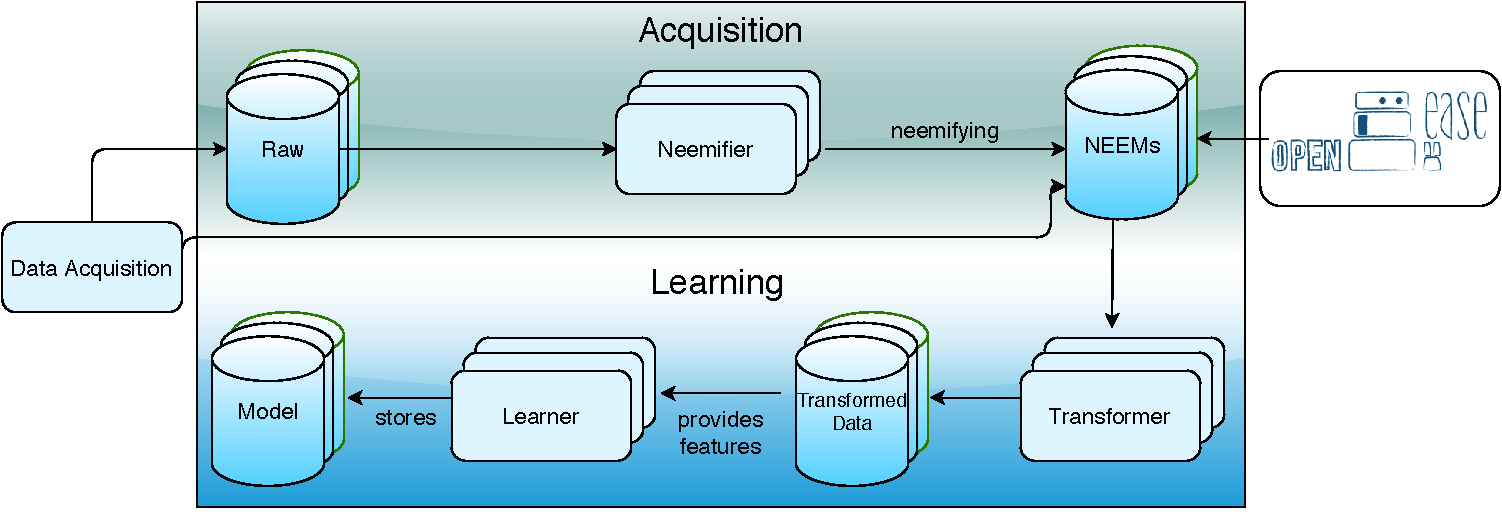
\includegraphics[width=\linewidth]{img/NEEM-Hub.pdf}
	\caption{The NEEM-Hub Architecture}
	\label{fig:neem-hub}
\end{figure} 


Currently, we are only supporting the upload and hosting from data, like raw data, \neems and processed data.
In future, we will provide the feature to share your Neemifier and Transformers with the community and create your own pipelines directly on the \neemhub.
In the rest of this section we will describe how you can upload the \neems to the \neemhub.

\section{Prerequisite}
\begin{enumerate}
	\item Due to security reasons our Hadoop Cluster can be only accessed via the University's intranet right now.	
	\item To support version control with our \neems we have the Install DVC https://dvc.org/ and get familiar with the tool https://dvc.org/doc/start.
	\item Install Hadoop or a client which can interact with our HDFS filesystem. 
	\item To be able to publish your data, you are required to have a git account on our GitLab system
	\url{https://neemgit.informatik.uni-bremen.de} .
	\item To test if you setup your system successful, you can try to download the following \neems : \url{https://neemgit.informatik.uni-bremen.de/neems/ease-2020-pr2-setting-up-table} .
\end{enumerate}


\section{Publishing}
At the time of writing this document, we are intending to host 3 groups of data:
\begin{description}
	\item[Raw data]
		We define might be data which cannot be captured directly as NEEMs during the acquisition.
	\item[\neems] 
	\item[Processed Data]
\end{description}

In the future, you will be able to publish your transformers which transform raw data into \neems or the \neems into processed data.
This will allow to share your tools easily with the community and also automatize data transformation pipeline.

\section{Maintaining}

